\chapter{Przerzutnik D jednozboczowy}

\section{Budowa układu}

\begin{itemize}
    \item Należało zbadać przerzutnik jednozboczowy D korzystając z układu 7474 (\ref{link:7474}).
        \begin{figure}[H]
            \centering
            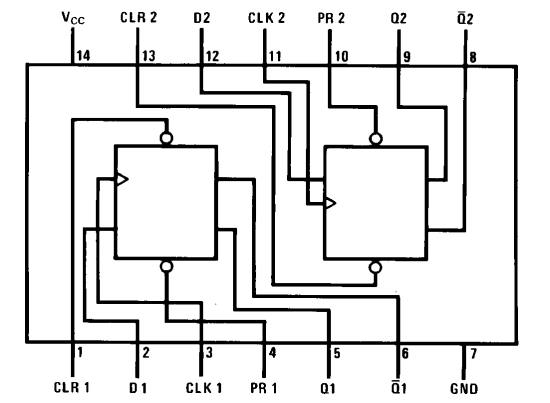
\includegraphics[width=0.8\textwidth]{img/schemes/7474_pins.png}
            \caption{Piny TTL 7474}
            \label{D_jednozboczowy:piny}
        \end{figure}
    \item Zgodnie z dokumentacją (\ref{link:7474}) jest to przerzutnik wyzwalany zboczem narastającym (0$\uparrow$)
    \item Na wejście CLR1 (pin 1) oraz PR (pin 4) podpięto logiczną 1 lub 0, korzystając z pinów 5V oraz 0V na płytce oraz rezystorów 1k$\Omega$ oraz 400$\Omega$ analogicznie jak w przerzutniku RS.
    \item Korzystając z jednego z impulsatorów (górnego) podajemy wartości na wejście D przerzutnika.
    \item Drugi z impulsatorów (dolny) służy jako zegar.
    \item Wyjście przerzutnika \textbf{Q} oraz $\overline{\textbf{Q}}$ (piny 5, 6) zostały wyprowadzone do diod elektroluminescencyjnych znajdujących się na prawej stronie płytki.
        \begin{figure}[H]
            \centering
            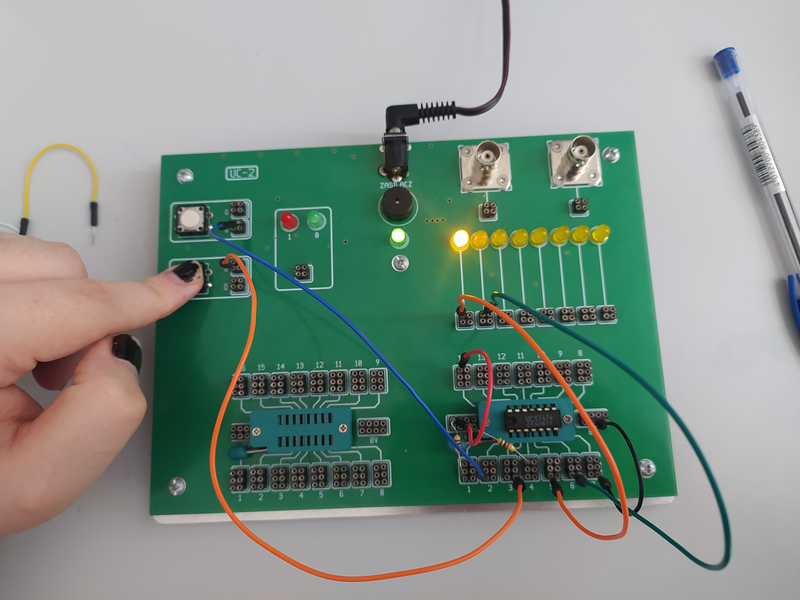
\includegraphics[width=0.7\textwidth]{img/5_2/1653500525143_scaled.png}
            \caption{Zbudowany przerzutnik D}
            \label{D_jednozboczowy:zbudowany}
        \end{figure}
        
        \begin{figure}[H]
            \centering
            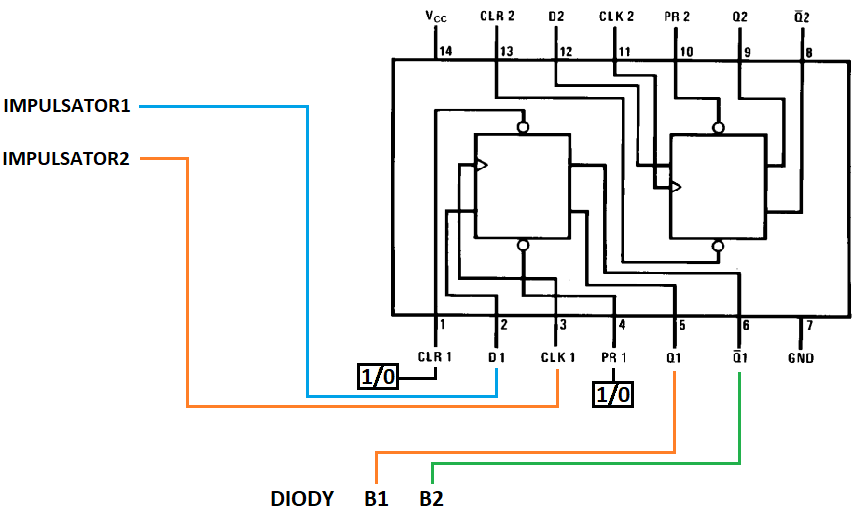
\includegraphics[width=\textwidth]{img/schemes_w_pins/5_2_w_pins.png}
            \caption{Schemat z połączonymi pinami}
            \label{D_jednozboczowy:schemat_z_pinami}
        \end{figure}
\end{itemize}

\pagebreak

\section{Testowanie układu}

\begin{itemize}
    \item Tabela wartości logicznych dla różnych wartości CLR oraz PR:
        \begin{figure}[H]
            \centering
            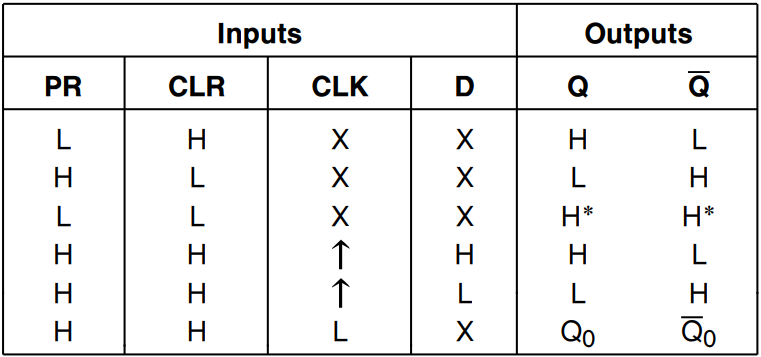
\includegraphics[width=0.7\textwidth]{img/schemes/5_2_table.png}
            \label{D_jednozboczowy:tablica_prawdy}
        \end{figure}
    \item Przerzutnik został przetestowany dla różnych wartości CLR oraz PR podpiętych do logicznej 1 lub 0 analogicznie jak wcześniej.
        \begin{figure}[H]
            \centering
            \begin{subfigure}[H]{0.4\textwidth}
                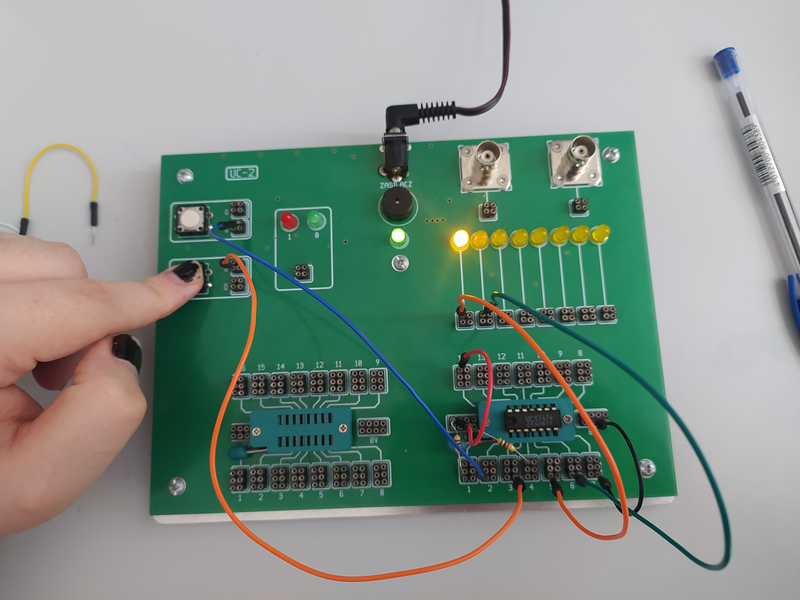
\includegraphics[width=\textwidth]{img/5_2/1653500525143_scaled.png}
            \end{subfigure}
            \begin{subfigure}[H]{0.4\textwidth}
                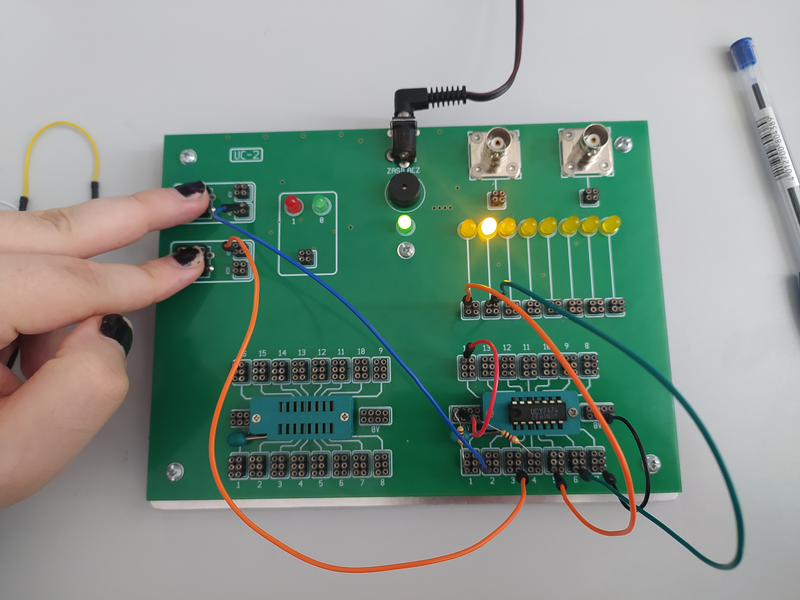
\includegraphics[width=\textwidth]{img/5_2/1653500525121_scaled.png}
            \end{subfigure}
            \begin{subfigure}[H]{0.4\textwidth}
                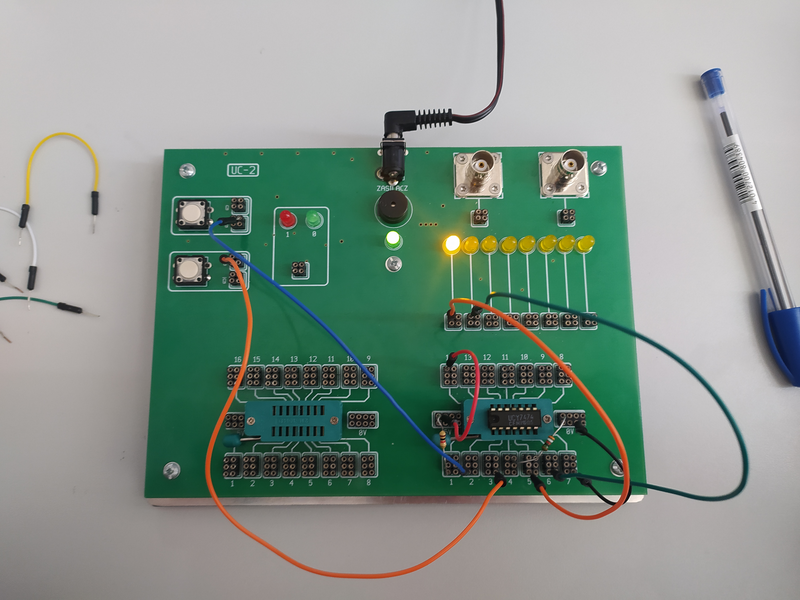
\includegraphics[width=\textwidth]{img/5_2/1653500525099_scaled.png}
            \end{subfigure}
            \begin{subfigure}[H]{0.4\textwidth}
                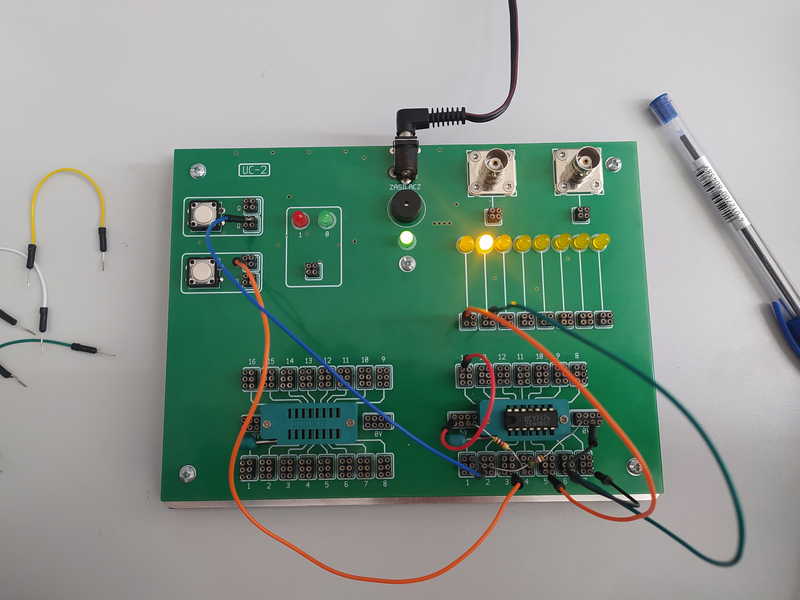
\includegraphics[width=\textwidth]{img/5_2/1653500525073_scaled.png}
            \end{subfigure}
            \caption{Testowanie przerzutnika D}
        \end{figure}
    \item Uzyskane wartości wyjść dla testowanych wartości CLR oraz PR zgadzały się z wartościami teoretycznymi. Układ działał \textbf{poprawnie}.
\end{itemize}